\documentclass[tikz,border=5pt]{standalone}
\usepackage{sansmath}
\usepackage{siunitx}

\begin{document}
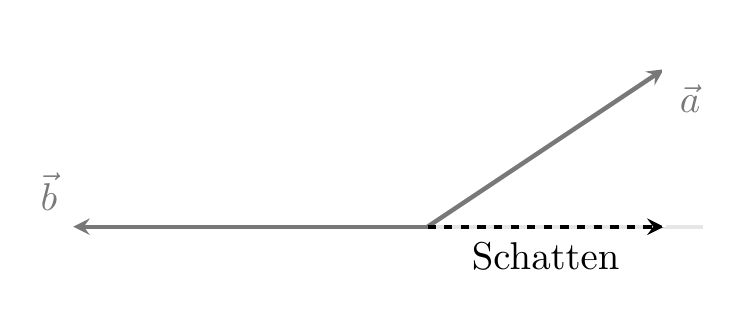
\begin{tikzpicture}

\def\size{3}
\def\textsize{1.4}
\definecolor{lightgray}{RGB}{120,120,120}
\definecolor{brightgray}{RGB}{230,230,230}
\coordinate (center) at (0, 0);

\draw[ultra thick, ->, >=stealth, lightgray] (center) -- (3, 2) node[below right, scale=\textsize] {$\vec{a}$};

\draw[ultra thick, ->, >=stealth, lightgray] (center) -- (-4.5, 0) node[above left, scale=\textsize] {$\vec{b}$};

\draw[ultra thick, brightgray] (center) -- (3.5, 0);

\draw[dashed, ultra thick, ->, >=stealth] (center) -- node[below, scale=\textsize] {Schatten}  (3, 0);

\draw[ultra thick, ->, >=stealth, white] (0.5, 2.5) -- (0.5, 0.66);
\draw[ultra thick, ->, >=stealth, white] (1.5, 2.5) -- (1.5, 1.33);
\draw[ultra thick, ->, >=stealth, white] (2.5, 2.5) -- (2.5, 2);

\draw[ultra thick, dashed, white] (3, 2) -- (3, 0);

\end{tikzpicture}
\end{document}